\chapter{Shared file systems using Manila}\label{cha:shared-file-systems}
OpenStack's Manila service makes it possible to create and manage
shared \gls{nfs} file systems for virtual machines.  This service is
not automatically enabled in the VSC cloud, so you should contact
\cloudinfo if you want to use shared file systems in your project.

\section*{Creating a Shared File System}\label{sec:creating-shared-file}
Creating a shared file system using the Horizon interface is quite straightforward:
\begin{enumerate}
\item Open the Share tab, and click Shares.  A list of existing shares (if any) is shown.
\item Click the \textbf{Create Share} button to open the following dialog:
  \begin{center}
    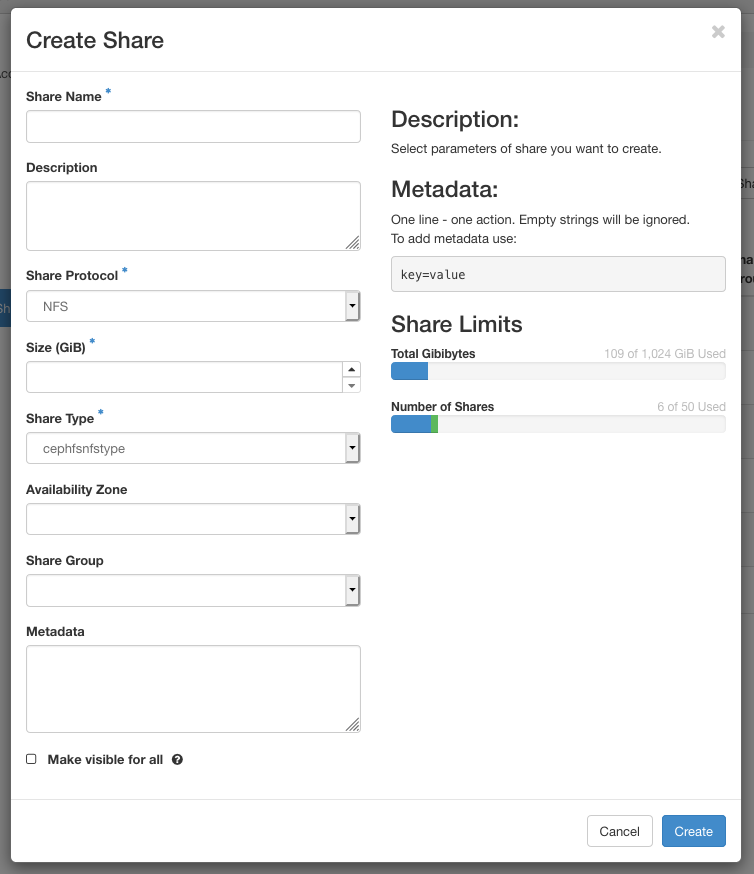
\includegraphics[width=0.7\textwidth]{img/create_share}
  \end{center}
  Fill out the following fields:
  \begin{description}
  \item[Share Name] Choose a name.
  \item[Description] Optionally, add a description.
  \item[Share Protocol] Use the default \gls{nfs} protocol.
  \item[Size (GiB)] Set the size of the shared file system to be
    created.  The total available storage and the amount currently
    used are shown on the right.
  \item[Share Type] Here, you must select ``cephfsnfstype'' (the only choice).
  \item[Metadata] You can attach additional metdata to your shared
    file system, which can be queried later on.
  \end{description}
  Other fields are not mandatory.  By default, the shared file system
  will only be visible within the current project (Visibility:
  ``private'').  Be careful with the option ``Make visible for all':
  enabling it will set the visibility of your shared file system to
  ``public'', making it visible for any other project in the VSC cloud
  as well.
\item Click \textbf{Create} to complete this step.
\end{enumerate}
% https://docs.openstack.org/security-guide/shared-file-systems/share-acl.html

At this point, the shared file system exists within OpenStack, but it cannot be used until we define access rules for it.

\section*{Defining \gls{nfs} access rules}\label{sec:defin-nfs-access}
You must define rules that define which machines on the network may
obtain read or write access to your shared file system.  By default,
in absence of any rules, a shared file system cannot be accessed by
anyone.

%TODO screenshots?
\begin{enumerate}
\item Open the drop-down menu in the \textbf{Actions} column for your share, and click \textbf{Manage Rules}.
\item You can now see all Share Rules for this shared file system.
  For a newly created file system, the list will be empty.  Click \textbf{Add rule}.
\item Fill out the \textbf{Add Rule} dialog:
  \begin{description}
  \item[Access Type] Only ``ip'' is supported.
  \item[Access Level] Choose if you want to give read and write
    (``rw'') or read-only (``ro'') permission with this rule.
  \item[Access To] Here, you can specify an ip address, or an address
    range, to which the rule applies.  The addresses should be
    specified according to the format expected by an NFS exports
    configuration file.  The following table contains a few examples,
    where it is assumed that the project's \_nfs network has the
    address range 10.10.x.0/24:

    \begin{tabular}{>{\bfseries}lp{0.7\textwidth}}
      10.10.x.13 & Allow this single ip address.
      \\ \hline
      0.0.0.0/0 & Allow any ip address.
      \\ \hline
      10.10.x.0/24 & Allow any ip address from the project's \_nfs network.  For a non-public shared file system this has the same effect as the previous rule, because such a shared file system can only be accessed from within our project's \_nfs network anyway.
      \\ \hline 
      10.10.x.0/28 & Allow addresses 10.10.x.0 until 10.10.x.15.
      \\
    \end{tabular}

  \end{description}
  Click \textbf{Add} to add the rule.
\end{enumerate}
Your rule now appears in the list.  You can add as many rules as you
wish, to set the access level for different addresses or address
ranges.

\section*{Accessing a shared file system}\label{sec:access-shar-file}
When the proper access rules for the shared file system are in place,
you can access it from an instance with a matching ip.  In order to be
able to mount the shared file system, your instance needs
\begin{itemize}
\item a \gls{nfs} client, installed by default on images provided by
  the VSC cloud, and
\item access to the \_nfs network.  Because your instance likely has to
  connect to the \_vm network as well, your VM should have two
  \gls{nic}'s.  Again, this is taken care of in the default images.
\end{itemize}

When you are ready to mount the network file system on an instance,
look up the network location of your file system using the Dashboard:
\begin{enumerate}
\item Open the Share tab and click Shares.  The list of all shared file systems in your project is shown.
\item Click the name of the shared file system you wish to access.
\item In the section ``Share Overview'', look for the item \textbf{Export locations}.
\item Copy the content of the \textbf{Path:} field.
\end{enumerate}

Once you know the location of your shared file system, you can mount
it on any VM with the appropriate access rights, e.g.\ for a shared
file system with location
\lstinline{10.2.0.2:/volumes/_nogroup/918...a78:}

\begin{prompt}
  %\shellcmd{sudo mount 10.2.0.2:/volumes/\_nogroup/918..a78 /mnt}
\end{prompt}
%%% Local Variables:
%%% mode: latex
%%% TeX-master: "intro-Cloud"
%%% End:
